% LearnMate -- ACL/EMNLP System Demonstrations submission.
%
% Build:   cd paper && latexmk -pdf main.tex
% Numbers: every figure quoted in the text is a \val{Name} macro defined in
%          tables/numbers.tex, which integrated-backend/eval/tables.py writes from the
%          result files of the evaluation scripts. An undefined one prints as ??.
%          Tables are \input only when their file exists.
%
% Demo tracks review single-blind: author names are shown, hence [final] rather than
% [review]. Check the current call before submitting.
\documentclass[11pt]{article}
\usepackage[final]{acl}
\usepackage{times}
\usepackage{latexsym}
\usepackage[T1]{fontenc}
\usepackage[utf8]{inputenc}
\usepackage{microtype}
\usepackage{inconsolata}
\usepackage{graphicx}
\usepackage{booktabs}
\usepackage{amsmath}
\usepackage{xcolor}
\usepackage{tikz}
\usetikzlibrary{positioning,shapes.geometric,arrows.meta,calc}

\IfFileExists{tables/numbers.tex}{\input{tables/numbers.tex}}{}
\newcommand{\val}[1]{\ifcsname #1\endcsname\csname #1\endcsname\else\textbf{??}\fi}
\newcommand{\tbl}[1]{\IfFileExists{tables/#1.tex}{\input{tables/#1.tex}}{\textit{[pending: run eval]}}}
\newcommand{\sys}{\textsc{LearnMate}}

\title{\sys: A Fully Local Study Assistant That Scales to the Classroom}

% TODO(authors): full names, affiliations and emails of every author.
\author{Dinura Ginige \and Co-author~Name \and Co-author~Name \\
  Department, University (TODO) \\
  \texttt{dinura1ginige@gmail.com}}

\begin{document}
\maketitle

\begin{abstract}
Study assistants built on local language models keep students' notes and questions on
hardware the institution controls, but they are designed for one student at a time: a
turn takes tens of seconds on a laptop, retrieval rests on heuristics, and nothing is
learned from the class as a whole. We present \sys{}, an open-source retrieval-augmented
study assistant that runs entirely on local models and treats a class sharing the same
course notes as an asset rather than a load. Four components make this work:
(1)~hybrid retrieval computed inside the vector database, with BM25 weighting and reciprocal
rank fusion in a single query;
(2)~a \emph{verified} answer cache that reuses an answer the system's LLM judge accepted
only when a duplicate-question cross-encoder confirms two students asked the same thing;
(3)~a lease-based job queue on MongoDB feeding continuously batched llama.cpp servers; and
(4)~confusion mining, which clusters every student's questions about a document and maps
them onto its pages under $k$-anonymity.
On eight chapters of an open law textbook and a simulated class of \val{WorkloadStudents}
students, server-side hybrid retrieval raises nDCG@10 after reranking from
\val{IRLegacyNdcg} to \val{IRRrfNdcg}, the verified cache serves reused answers with
\val{CachePrecision}\% precision where an embedding threshold alone reaches
\val{CacheEmbPrecision}\%, and question mining attributes \val{HeatAttribution}\% of
questions to the right page.
\end{abstract}

\section{Introduction}

Large language models can explain, quiz and summarise course material on demand
\citep{kasneci2023chatgpt}, and retrieval-augmented generation \citep{lewis2020rag} lets
them answer from a student's own notes rather than from memory. Running the models locally
keeps those notes and questions private, which matters to institutions that cannot send
student data to a third party. The price is speed and scale: on a laptop CPU, one grounded
answer from a 3B-parameter model takes 30--60 seconds, and a single model instance serves
one student at a time.

\sys{} started as such a single-student assistant. Its documents are stored by the
SHA-256 of their bytes, however, and that detail changes the picture. When a class uploads
the same lecture notes, every student is talking to the \emph{same} document -- one index,
and, during revision, largely the same questions. This paper describes four additions that
exploit that sharing, and the evaluation harness that measures them:

\begin{itemize}\setlength\itemsep{0pt}
\item \textbf{Server-side hybrid retrieval.} Stemmed BM25 whose inverse document frequencies
  are kept by the vector database, fused with dense retrieval by RRF inside one tenant-filtered
  query, replacing an unfused union with an in-process BM25 index (\S\ref{sec:retrieval}).
\item \textbf{Verified answer reuse.} A semantic cache of judge-accepted answers shared
  across students, in which a cross-encoder must confirm that two questions are duplicates
  before an answer is reused (\S\ref{sec:cache}).
\item \textbf{Scalable serving.} A MongoDB job queue with atomic claims and renewable leases,
  a pool of workers, and continuously batched model servers (\S\ref{sec:serving}).
\item \textbf{Confusion mining.} A per-document heatmap of where a class struggles, mined
  from every student's questions with aggregation pipelines, HDBSCAN and class-based
  TF-IDF, and shown only above a $k$-anonymity floor (\S\ref{sec:mining}).
\end{itemize}

\noindent Everything runs on local models: Qwen2.5-3B \citep{qwen2025qwen25} writes answers,
Llama-3.2-3B \citep{grattafiori2024llama3} judges them (a different model family, so the
judge does not favour its own style), MiniLM \citep{wang2020minilm,reimers2019sbert} embeds,
and a MiniLM cross-encoder reranks \citep{nogueira2019passage}. Code, the evaluation
harness and a screencast are available.\footnote{TODO(authors): repository URL and video link.}

\begin{figure*}[t]
\centering
% System architecture. Blue boxes are the four components this paper adds.
% Three rows on a fixed grid: request path, turn pipeline, stores and model servers.
\resizebox{\textwidth}{!}{%
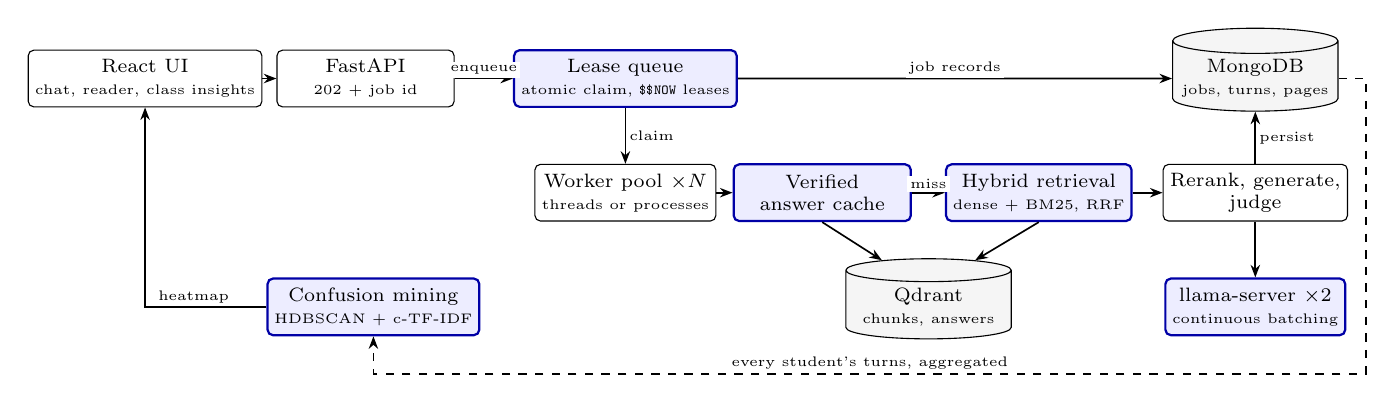
\begin{tikzpicture}[
    font=\scriptsize,
    box/.style={draw, rounded corners=2pt, align=center, minimum height=0.72cm,
                minimum width=2.25cm, inner sep=2.5pt, fill=white},
    new/.style={box, draw=blue!65!black, fill=blue!7, thick},
    store/.style={draw, cylinder, shape border rotate=90, aspect=0.16, align=center,
                  minimum height=0.85cm, minimum width=2.1cm, inner sep=2pt, fill=gray!8},
    arr/.style={-{Stealth[length=1.6mm]}, semithick},
    lbl/.style={font=\tiny, inner sep=1.2pt, fill=white},
]
% Row 1: the request path.
\node[box]   (ui)    at (0, 0)     {React UI\\\tiny chat, reader, class insights};
\node[box]   (api)   at (2.8, 0)   {FastAPI\\\tiny 202 + job id};
\node[new]   (queue) at (6.1, 0)   {Lease queue\\\tiny atomic claim, \texttt{\$\$NOW} leases};
\node[store] (mongo) at (14.1, 0)  {MongoDB\\\tiny jobs, turns, pages};

% Row 2: one chat turn, left to right.
\node[box]   (work)  at (6.1, -1.45)  {Worker pool $\times N$\\\tiny threads or processes};
\node[new]   (cache) at (8.6, -1.45)  {Verified\\answer cache};
\node[new]   (retr)  at (11.35, -1.45) {Hybrid retrieval\\\tiny dense + BM25, RRF};
\node[box]   (gen)   at (14.1, -1.45) {Rerank, generate,\\judge};

% Row 3: stores, servers and the miner.
\node[new]   (mine)   at (2.9, -2.9)   {Confusion mining\\\tiny HDBSCAN + c-TF-IDF};
\node[store] (qdrant) at (9.95, -2.9)  {Qdrant\\\tiny chunks, answers};
\node[new]   (llama)  at (14.1, -2.9)  {llama-server $\times 2$\\\tiny continuous batching};

% Request path.
\draw[arr] (ui) -- (api);
\draw[arr] (api) -- node[lbl, above] {enqueue} (queue);
\draw[arr] (queue) -- node[lbl, above] {job records} (mongo);
\draw[arr] (queue) -- node[lbl, right] {claim} (work);

% The turn.
\draw[arr] (work) -- (cache);
\draw[arr] (cache) -- node[lbl, above] {miss} (retr);
\draw[arr] (retr) -- (gen);
\draw[arr] (gen) -- (llama);
\draw[arr] (gen) -- node[lbl, right] {persist} (mongo);
\draw[arr] (cache.south) -- (qdrant.north west);
\draw[arr] (retr.south) -- (qdrant.north east);

% Mining reads the turns and feeds the UI.
\draw[arr, dashed] (mongo.east) -- ++(0.35, 0) |- (2.9, -3.75)
    node[lbl, pos=0.75, above] {every student's turns, aggregated} -- (mine.south);
\draw[arr] (mine.west) -| node[lbl, pos=0.3, above] {heatmap} (ui.south);
\end{tikzpicture}}

\caption{\sys{} architecture. A chat turn is a job: the API enqueues it, a worker claims it
under a lease and runs the turn graph (rewrite $\to$ cache lookup $\to$ hybrid retrieval
$\to$ rerank $\to$ generate $\to$ judge $\to$ persist $\to$ cache store). Blue boxes are the
components added in this work.}
\label{fig:arch}
\end{figure*}

\section{System Overview}
\label{sec:overview}

A student uploads a PDF, Word, PowerPoint or \LaTeX{} file. Ingestion extracts and cleans
the text, removes running headers, splits it into chunks of at most 900 characters that
never cross a page boundary, embeds them, and stores the chunks in Qdrant
\citep{qdrant2023} and the pages, files and all history in MongoDB. The workspace
(Figure~\ref{fig:screens}) shows the document beside two panels: a generator for key
points, summaries and multiple-choice or short-answer questions, and a chat. Each chat turn
is a LangGraph state machine (Figure~\ref{fig:arch}): a follow-up is rewritten into a
standalone question; retrieval returns candidates that a cross-encoder reranks to three;
if the best scores at least $0.5$ the answer is written from those chunks with page
citations, otherwise the assistant says it is answering from general knowledge. The judge
scores grounded answers from 1 to 100 against the retrieved text; a score under 70 triggers
one regeneration with the judge's critique, and the better of the two attempts is kept.
Everything slow runs as a background job that the browser polls, with the answer streamed
into the job record as it is written.

\section{Scaling to the Classroom}

\subsection{Hybrid retrieval inside the vector database}
\label{sec:retrieval}

The original retriever took the top 15 dense hits and the top 10 hits of an in-process
BM25 index and returned their union, unfused, for the reranker. The BM25 index lived in
each server process, was rebuilt from MongoDB on first use, and scored every chunk of the
document on every query.

\sys{} now computes both halves in Qdrant. Okapi BM25 \citep{robertson2009bm25} factors
into a document part -- the saturated, length-normalised term frequency
$\frac{tf(k_1+1)}{tf+k_1(1-b+b\,|d|/\overline{|d|})}$ -- and a query part, the inverse
document frequency. The first is computed at ingest and stored as a sparse vector over
Porter-stemmed \citep{porter1980}, stopword-filtered terms hashed to 31-bit ids; the second
is computed by the server from the collection's own statistics at query time (Qdrant's IDF
modifier), so no process holds corpus statistics. A query then issues one request with two
prefetches -- dense and sparse, each filtered to the student's document, which is the
collection's tenant key -- fused by reciprocal rank \citep[$k{=}60$;][]{cormack2009rrf}.
Because a fused score is a rank rather than a similarity, the fallback mode decision (used
if the reranker is unavailable) compares the chunk's own dense cosine, fetched alongside.
An existing collection is migrated by copying its dense vectors, without re-embedding.

\subsection{Verified answer reuse}
\label{sec:cache}

Semantic caches answer a new query with the response to a previous, similar one
\citep{bang2023gptcache,gill2025meancache}. Choosing the similarity threshold is the hard
part \citep{schroeder2025vcache}. Questions about the same passage share their content
words, and questions that differ only in \emph{advantages} vs.\ \emph{disadvantages}, or in a rule
vs.\ its exception, embed almost identically. A threshold loose enough to catch real
paraphrases therefore also serves wrong answers.

\sys{} separates shortlisting from deciding, as retrieval does. A lookup embeds the
student's standalone question and takes the three nearest cached questions for the same
document, generator, prompt version and index version (a re-ingested document invalidates
its answers). Candidates above a cosine threshold $\tau$ are read by a cross-encoder trained
on duplicate questions (\texttt{quora-distilroberta-base}), and a hit needs its
probability above a second threshold. Only answers the judge scored and accepted, in
grounded mode, and not produced by rewriting a follow-up, are stored; a hit returns the
answer with its citations and source chunks, and the interface labels it ``verified answer
reused''. Cache entries contain no user or session identifiers.

\subsection{Scalable serving}
\label{sec:serving}

The original server had one worker thread and an in-memory queue. That was correct, since
llama.cpp \citep{gerganov2023llamacpp} holds one context per model, but it serialised the
whole class. \sys{} makes the job records themselves the queue. A worker claims the oldest
due job with one atomic \texttt{find\_one\_and\_update} that stamps a lease with the
\emph{database's} clock (\texttt{\$\$NOW}), so workers on different machines agree on
expiry. It renews the lease every 15\,s, and writes a result only while it still holds the
lease. A reaper requeues jobs whose lease has lapsed, up to a retry budget, and a unique
index on (job, role) makes a retried turn's persistence idempotent. Any number of worker
threads and processes can share one database. The models move behind \texttt{llama-server}
with parallel slots, which interleaves the tokens of concurrent requests in shared forward
passes: continuous batching \citep{yu2022orca,kwon2023vllm}. The default configuration is
unchanged, and the pool is enabled with two settings.

\subsection{Confusion mining}
\label{sec:mining}

Because a document is shared, every question any student asks about it is evidence about
the document. Two MongoDB aggregation pipelines do the counting server-side: a
\texttt{\$setWindowFields} pass pairs each answer with the question before it, and a
\texttt{\$facet} computes per-page counts of questions, distinct students, answers written
from general knowledge, and low-scored answers. A question is attributed to the page of its
best citation. If the document could not answer it, it is attributed to the page retrieval
came nearest to, since that is the page that failed to answer it. Questions are embedded and clustered with
HDBSCAN \citep{campello2013hdbscan,mcinnes2017hdbscan}, which finds the number of topics
itself and leaves one-off questions as noise, and each topic is labelled by class-based
TF-IDF, following BERTopic \citep{grootendorst2022bertopic}. A page's confusion combines its
share of questions with four signals: answered from general knowledge, scored low,
delivered below the pass mark, and the same student returning to the same topic within a
week. Pages and topics that fewer than $k{=}3$ students contributed to are suppressed
\citep{sweeney2002kanon}, and only keywords are shown, never questions. Clicking a page in
the heatmap opens it in the reader.

\begin{figure}[t]
\centering
\IfFileExists{figures/screens/workspace.png}{%
  \includegraphics[width=\columnwidth]{figures/screens/workspace.png}}{%
  \fbox{\parbox[c][3.2cm][c]{0.92\columnwidth}{\centering\small [screenshot: workspace with
  class-insights heatmap and a reused answer]}}}
\caption{The workspace: the document (left) and the class-insights heatmap (right). Darker
pages drew more questions that landed badly, and hatched pages had fewer than $k$ students.
Clicking a page opens it in the reader.}
\label{fig:screens}
\end{figure}

\section{Demonstration}

The demonstration follows two students through one chapter. Student~A uploads the chapter
and asks what makes a contract enforceable; the answer streams in with page citations while
the judge reviews it. Student~B uploads the same file (it is recognised by hash and not
re-processed) and asks the question in other words; the answer appears immediately, marked
as a verified reuse, and hovering the badge shows the similarity and verifier scores. Asking
instead about the \emph{exception} to the rule is not served from the cache. The instructor's
view is the class-insights tab: the heatmap after a simulated fortnight of forty students,
the topics they asked about, and a page that the chapter explains poorly; clicking the page opens
it. Finally, a terminal shows two worker processes draining the queue; one is killed
mid-answer, its lease lapses, and the other finishes the turn.

\section{Evaluation}
\label{sec:eval}

\paragraph{Setup.} The corpus is \val{CorpusDocs} chapters (\val{CorpusPages} pages,
\val{CorpusChunks} chunks) of an open law textbook \citep{valbrune2019bizlaw}, each ingested as
one shared document. Following InPars and Promptagator
\citep{bonifacio2022inpars,dai2023promptagator}, the local generator wrote, for each of
\val{WorkloadFamilies} sampled chunks, a question the chunk answers, two paraphrases of
it, and a near-miss (a question on the same topic needing a different answer): in total
\val{WorkloadQuestions} questions with a known source chunk. A simulated class of
\val{WorkloadStudents} students then asks \val{WorkloadAsks} questions over two weeks,
choosing questions by a Zipf distribution and wordings at random. One chapter is used for
tuning, and results are reported on the other seven. Unless stated otherwise, times are from a CPU-only laptop
(\val{TurnMachine}).

% EVALUATION-PROSE: written after the results are in (see integrated-backend/eval).

\paragraph{Retrieval.}
\begin{table}[t]
\centering\small\setlength\tabcolsep{3pt}
\resizebox{\columnwidth}{!}{\tbl{ir}}
\caption{Retrieval over \val{IRQueries} questions (seeds and paraphrases): Recall@3 (what
reaches the prompt) and graded nDCG@10, before and after reranking, and first-stage
latency.}
\label{tab:ir}
\end{table}

\paragraph{Answer reuse.}
\begin{table}[t]
\centering\small\setlength\tabcolsep{4pt}
\resizebox{\columnwidth}{!}{\tbl{cache}}
\caption{Cache decisions on held-out chapters: paraphrases should hit their own question's
entry, near-misses should miss. Thresholds chosen on the development chapter.}
\label{tab:cache}
\end{table}

\paragraph{Serving.}

\paragraph{Confusion mining.}
\begin{table}[t]
\centering\small
\tbl{heatmap}
\caption{Question mining against the simulated class's known topics and source pages.}
\label{tab:heatmap}
\end{table}

\section{Related Work}

Hybrid lexical-dense retrieval and its fusion functions are well studied
\citep{cormack2009rrf,bruch2023fusion,thakur2021beir}, as are learned sparse
representations \citep{formal2021splade}; \sys{} contributes an engineering point: that the
whole of BM25 can live in the vector database next to the dense index, sharing its tenant
filter. Semantic caches \citep{bang2023gptcache,gill2025meancache} trade freshness for
latency. vCache \citep{schroeder2025vcache} learns per-entry thresholds with an error
guarantee. \sys{} instead verifies each candidate with a cross-encoder and caches only
answers an LLM judge accepted \citep{zheng2023judge}, so a reused answer has been checked
twice. Continuous batching \citep{yu2022orca,kwon2023vllm} is standard in GPU serving; we
show the queue design that lets a local deployment use it. Confusion in course forums has
been detected from posts \citep{yang2015confusion} and surfaced on learning-analytics
dashboards \citep{verbert2013dashboards}; \sys{} mines the questions students already ask
an assistant, grounded in the pages of the notes they share. RAG evaluation frameworks
\citep{es2024ragas} score answers; our harness scores the systems components.

\section{Conclusion}

\sys{} turns a class sharing course notes into shared retrieval, shared verified answers,
shared serving capacity and shared insight, without data leaving local hardware. Every
number above is produced by a script in the repository, with the commit and machine
recorded alongside it.

\section*{Limitations}

The questions are LLM-generated and the class is simulated. Generated questions share
vocabulary with their source chunk, which favours lexical retrieval, so we report
paraphrases separately, and the simulation has no judge scores, so two of the four
confusion signals are absent from the mining evaluation. The corpus is one English law
textbook. BM25's IDF is collection-wide and its average length fixed at index time. The
duplicate-question verifier was trained on general web questions, not legal ones. Latency
figures come from a single machine. No real students took part. A classroom study is
the necessary next step.

\section*{Ethics Statement}

All models run locally; no student text leaves the deployment. Cache entries hold no
user or session identifiers, and the confusion heatmap shows only aggregates above a
$k$-anonymity floor and never question text, though aggregates about small classes can
still be revealing and $k$ should be set with that in mind. A reused answer is labelled
as such. The corpus is used under its CC BY-NC-SA 4.0 licence for non-commercial research
and is not redistributed.

\bibliography{references}

\end{document}
